\documentclass{beamer}
\usetheme{metropolis}           % Use metropolis theme
\usecolortheme{beaver}
\setbeamerfont{caption}{size=\scriptsize}
\title{Charla GitHub avanzado 2024}
\subtitle{Ramas, comunicación, workflows}
\date{202224}
\author{Alejandro Barrachina Argudo}
\institute{Universidad Complutense de Madrid}
\begin{document}
\maketitle

\begin{frame}{Tabla de contenidos}
    \tableofcontents
\end{frame}

\AtBeginSection[]{
    \begin{frame}{Tabla de contenidos}
        \tableofcontents[currentsection]
    \end{frame}
}
\AtBeginSubsection[]{
    \begin{frame}{Tabla de contenidos}
        \tableofcontents[currentsubsection]
    \end{frame}
}
\section{Introducción}
\begin{frame}{Introducción}

    Charla anterior: \url{https://github.com/ALK222/charla-git-principiantes-2023}
    
    Se asume que:
    \begin{itemize}
        \item Tenéis cuenta de GitHub
        \item Sabéis hacer crear repositorios
        \item Sabéis hacer \textit{commit}, \textit{push}, \textit{pull}
    \end{itemize}
\end{frame}

\section{Ramas}
\begin{frame}{Ramas}
    \begin{itemize}
    \item Mantienen el desarrollo paralelo para distintas partes del programa

    \item Mantienen separadas las versiones estables de las de desarrollo
     
    \item Nos permiten proteger ciertas ramas
\end{itemize}

\end{frame}

\begin{frame}
    \begin{figure}[H]
        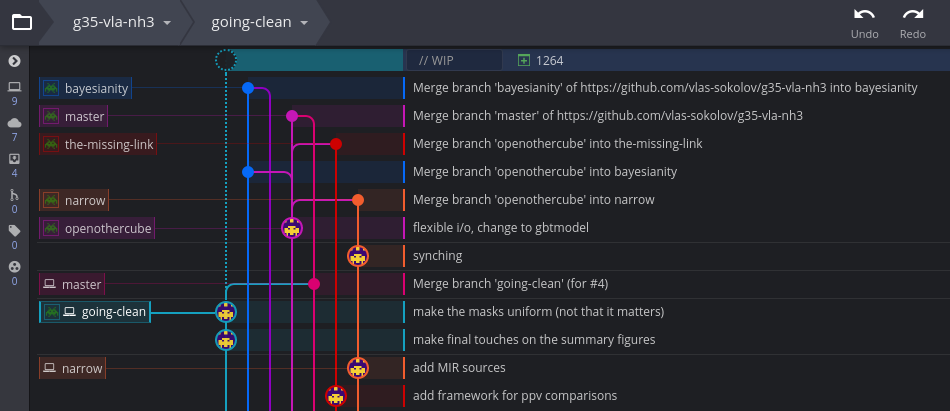
\includegraphics[width=0.7\textwidth]{Images/ejemplo-ramas.png}
        \caption{origen de la imagen: \url{https://stackoverflow.com/questions/46827112/toggling-branch-tree-view-in-gitkraken}}
    \end{figure}
\end{frame}
\subsection{Ramas - Main}
\begin{frame}{Main}

    

\end{frame}

\end{document}